\documentclass{article}
\usepackage[utf8]{inputenc}
\usepackage{graphicx}
\title{TUGAS DATABASE 2}
\author{Gharrieb Nouvaldi (1184082) }
\date{1 November 2019}

\begin{document}

\maketitle

\par
Langkah-langkah Pembuatan Aplikasi Oracle APEX
\begin{enumerate}
    \item Langkah Pertama kita melakukan Login untuk mengakses web Oracle Apex.
    \begin{figure}[h]
	\centering
	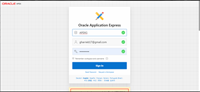
\includegraphics[width=6cm]{Figure/Login.png}
	\caption{Login}
	\label{fig:gambar}
	\end{figure}

    \item Langkah selanjutnya pilih "App Builder"  klik "Create"
    \begin{figure}[h]
	\centering
	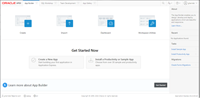
\includegraphics[width=4cm]{Figure/Create.png}
	\caption{Create}
	\label{fig:gambar}
	\end{figure}

    \item Setelah itu kalian klik "From a File"
    \begin{figure}[h]
	\centering
	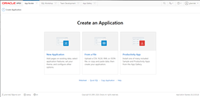
\includegraphics[width=5cm]{Figure/FOF.png}
	\caption{From a File}
	\label{fig:gambar}
	\end{figure}

    \item Lalu Masukkan file yang akan kalian pakai, ada dua cara yang dapat anda gunakan, cara yang pertama dengan melakukan "Upload File". Cara yang kedua melakukan "Copy and Paste". Saya disini memakai cara yang ke dua dengan melakukan "Upload File" file yang akan kita dibuat.
     \begin{figure}[!htbp]
        \centering
        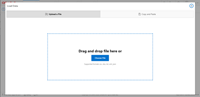
\includegraphics [width=5cm]{Figure/CF.png}
        \caption{Caption}
        \label{capture3}
    \end{figure}
    
    \item Selanjutnya isi "Table Name" yang akan kalian buat, untuk eror tabel name atau "Table Name Error" akan otomatis terisi jika telah mengisi "Table Name". Jika sudah lalu klik "Load Data"
    \begin{figure}[h]
	\centering
	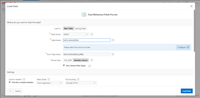
\includegraphics[width=7cm]{Figure/ID.png}
	\caption{Create}
	\label{fig:gambar}
	\end{figure}
	
    \item Setelah itu akan muncul "Load Data" tadi, maka akan ada ceklis hijau lalu klik "View Table"
    \begin{figure}[h]
	\centering
	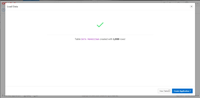
\includegraphics[width=6cm]{Figure/CA.png}
	\caption{Create}
	\label{fig:gambar}
	\end{figure}
	
	    \item Setelah dibuat, maka lakukan Run Application
    \begin{figure}[h]
	\centering
	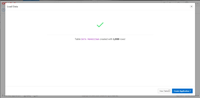
\includegraphics[width=5cm]{Figure/CA.png}
	\caption{Create}
	\label{fig:gambar}
	\end{figure}
    
    \item Sebelum masuk ke aplikasi yang telah dibuat tadi, kalian harus login terlebih dahulu memakai akun masuk oracle APEX
    \begin{figure}[h]
	\centering
	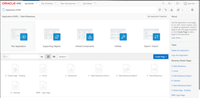
\includegraphics[width=5cm]{Figure/RA.png}
	\caption{Create}
	\label{fig:gambar}
	\end{figure}
    
    \item Setelah login maka akan masuk ke tampilan awal aplikasi yang telah dibuat tadi
     \begin{figure}[h]
	\centering
	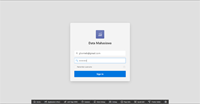
\includegraphics[width=5cm]{Figure/LRA.png}
	\caption{Create}
	\label{fig:gambar}
	\end{figure}
	
Data yang telah diinputkan sudah ternormalisasi, dengan menggunakan kolom yang sudah  disesuaikan, dengan karakter data masing-masing. Contohnya: data nama mahasiswa, semuanya terdapat pada kolom "NAMA"
     \begin{figure}[h]
	\centering
	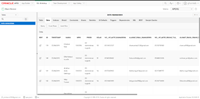
\includegraphics[width=8cm]{Figure/Norm.png}
	\caption{Create}
	\label{fig:gambar}
	\end{figure}

	
\end{enumerate}
\end{document}
